\documentclass[10pt]{beamer}
\usepackage[utf8]{inputenc}
\usepackage[T1]{fontenc}
\usepackage[slovene]{babel}
\usepackage{tikz}
\usepackage{quantikz}
\usepackage{amsmath}
\usepackage{physics}
\usepackage{graphicx}
\usepackage{circuitikz}
\usetikzlibrary{shapes}
% \usepackage{tikz-cd}
%\pgfdeclarelayer{nodelayer}
%\pgfdeclarelayer{edgelayer}
%\pgfsetlayers{nodelayer,edgelayer}

%\tikzcdset{every matrix/.style={ampersand replacement=\&}}

\usetheme{metropolis}

\definecolor{zx_red}{RGB}{232, 165, 165}
\definecolor{zx_green}{RGB}{216, 248, 216}
\definecolor{had_yellow}{RGB}{221, 218, 28}

\tikzstyle{gn}=[circle,rounded corners=0.8em,fill=zx_green,draw=black,
  line width=0.8 pt,inner sep=3pt,minimum width=1.5em,minimum height=1.5em]
\tikzstyle{rn}=[circle,rounded corners=0.8em,fill=zx_red,draw=black,
  line width=0.8 pt,inner sep=3pt,minimum width=1.5em,minimum height=1.5em]
\tikzstyle{had}=[rectangle,fill=had_yellow,draw=black,
  line width=0.8 pt,inner sep=3pt,minimum width=1.5em,minimum height=1.5em]
\tikzstyle{func}=[trapezium,draw=black,shape border rotate=270, 
line width=0.8 pt,inner sep=3pt,minimum width=1.4em,minimum height=1.2em]
\tikzstyle{classi}=[regular polygon, regular polygon sides = 3,draw=black, shape border rotate = 210,
line width=0.8 pt, inner sep=2pt,minimum width=1.5em,minimum height=1.5em]
\tikzstyle{classo}=[regular polygon, regular polygon sides = 3,draw=black, shape border rotate = 30,
line width=0.8 pt,inner sep=3pt,minimum width=1.5em,minimum height=1.5em]
\usepackage{appendixnumberbeamer}

\usepackage{booktabs}
\usepackage[scale=2]{ccicons}

\usepackage{pgfplots}
\usepgfplotslibrary{dateplot}

\usepackage{xspace}
\newcommand{\themename}{\textbf{\textsc{metropolis}}\xspace}

\title{ZX-račun}
\subtitle{Nov pristop h kvantnem računalništvu}
\date{\today}
\author{Tadej Petrič}
\institute{Fakulteta za matematiko in fiziko}
% prednosti kvantnega računalništva vs klasično
% kvantna mehanika
% klasično kvantno rač
% 4+ zx
\begin{document}
\begin{frame}
  \maketitle
\end{frame}
\begin{frame}
  \frametitle{Osnove klasičnega računalništva}
  \begin{itemize}
  \item Prisotna električna napetost ali pa ne
  \item Klasične vrednosti \(1\) in \(0\) (biti)
    \begin{itemize}
    \item Označimo \(\ket1\) in \(\ket0\), da razločimo od števil
    \end{itemize}
  \item Logična vrata \(\land\), \(\lor\), \(\lnot\)
  \item Bite lahko brišemo \(\ket0\land x \mapsto \ket0\)
  \item Bite lahko kopiramo (razcep žic)
  \item Stanje računalnika opišemo s skupino zaporednih bitov
    \begin{itemize}
    \item Primer \(\ket{00101} = (0,0,1,0,1)\)
    \item Na skupinah lahko uporabljamo logična vrata
    \end{itemize}
  \end{itemize}
\end{frame}
\begin{frame}
  \frametitle{Kubiti}
  \begin{itemize}
  \item Kubiti so kvantna verzija bitov
  \item Lahko mešanica \(\ket0\) in \(\ket1\)
  \item Predstavimo kot linearno kombinacijo \(a\ket0 + b\ket1\)
  \item Zahtevamo \(a^2+b^2 = 1\) kot robni pogoj
  \item Fizikalno ponavadi predstavimo s spinom delcov (navidezno vrtenje okoli (X,Y,Z) osi)
  \item Ko jih izmerimo, dobimo klasično vrednost \(\ket0\) ali \(\ket1\)\pause
    \begin{itemize}
    \item Vrednosti meritve ne vemo vnaprej
    \item Vemo le verjetnost, da izmerimo določeno vrednost
    \item Za meritvijo vrednost ostane ista
    \end{itemize}
  \end{itemize}
\end{frame}
\begin{frame}
  \frametitle{Skupine kubitov}
  \begin{itemize}
  \item Pomembni so sistemi večih kubitov
  \item Kubiti so med seboj lahko prepleteni
    \begin{itemize}
    \item Ko dobimo informacijo o kubitu, dobimo informacijo o kubitih, s katerimi je prepleten
    \end{itemize}\pause
  \item Primer \(\frac1{\sqrt2}(\ket{00}+\ket{11})\)
    \begin{itemize}
    \item Dva prepletena kubita\pause
    \item Na prvem izmerimo \(\ket0\) ali \(\ket1\) z enako verjetnostjo
    \item Če za tem izmerimo drugi kubit, bo z verjetnostjo \(1\) odgovor enak kot pri prvem
    \end{itemize}
  \end{itemize}
\end{frame}
\begin{frame}
  \frametitle{Kloniranje in brisanje}
  Lastnosti kvantnih vrat
  \begin{itemize}
  \item Kubitov ne moremo klonirati
    \begin{itemize}
    \item Ne obstajajo vrata \(\forall x.\, \ket{0x}\mapsto\ket{xx}\)
    \item Vrata bodo imela kvečjemu manj izhodov kot vhodov
    \end{itemize}\pause
  \item Kubitov ne moremo brisati
    \begin{itemize}
    \item Ekvivalentno prejšnji trditvi, če čas teče v preteklost
    \item Ne obstajajo vrata \(\forall x.\, \ket x\mapsto\ket0\)
    \item Vrata kvečjemu več izhodov kot vhodov
    \end{itemize}\pause
  \item Vrata enako število vhodov kot izhodov
  \end{itemize}
\end{frame}
\begin{frame}[fragile]
  \frametitle{Kvantna vezja}
  \begin{itemize}
  \item Kubite lahko predstavimo z vektorji dolžine \(1\) v bazi \(\ket0, \ket1\)
  \item Kvantna vrata predstavimo z unitarnimi preslikavami
  \end{itemize}
  Vezja lahko narišemo tudi z diagramom:\\
  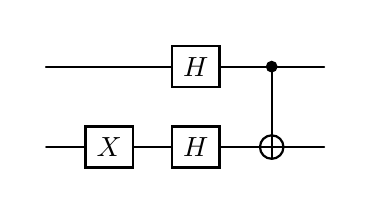
\begin{tikzpicture}
    \node[scale=1.0] {
      \begin{quantikz}
        \qw & \qw       & \gate{H} & \ctrl{1} & \qw \\
        \qw & \gate{X}  & \gate{H} & \targ{}  & \qw
      \end{quantikz}
    };
  \end{tikzpicture}\\
  Tukaj 3 unarna vrata (X, H) in ena binarna (C-NOT)
\end{frame}
\begin{frame}
  \frametitle{Težave}
  \pause
  \begin{itemize}
  \item Za večja vezja zelo nepregledna \pause
  \item Če dve vezji predstavljata isto transformacijo, ne poznamo (vedno) pravil, ki bi prvo pretvorila v drugo\pause
  \item Veliko trditev o kvantni mehaniki težko dokazati
  \end{itemize}
\end{frame}
\begin{frame}
  \frametitle{ZX-Račun}
  Vezje predstavimo kot graf. Definiramo dva tipa vozlišč: X pajek (rdeč) in Z pajek (zelen)\\
  Lahko imata poljubno število vhodov ali izhodov\\
  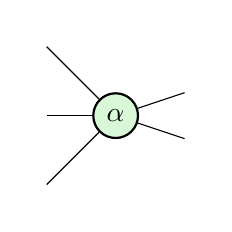
\begin{tikzpicture}
    %\begin{pgfonlayer}{nodelayer}
    \node (01) at (0, 0) {};
    \node (02) at (0, 1) {};
    \node (03) at (0, 2) {};
    \node [style=gn] (1) at (1.00, 1.00) {\(\alpha\)};
    \node (21) at (2, 0.66666) {};
    \node (22) at (2, 1.33333) {};
    %\end{pgfonlayer}
    %\begin{pgfonlayer}{edgelayer}
    \draw (01) to (1);
    \draw (02) to (1);
    \draw (03) to (1);
    \draw (1) to (21);
    \draw (1) to (22);
    %\end{pgfonlayer}
  \end{tikzpicture}\\
  Ta pajek ustreza preslikavi
  \begin{align*}
    \ket{00}\bra{000} + e^{i\alpha}\ket{11}\bra{111}
  \end{align*}
  Neformalno \(\bra{000}\) predstavlja kolikšen del vhoda je \(\ket{000}\)
\end{frame}
\begin{frame}
  \frametitle{Več o pajkih}
  Rdeč pajek (X) se obnaša podobno kot Z pajek, le da v bazi \(\{\ket{-},\ket{+}\}\) namesto \(\{\ket0,\ket1\}\)\\
  Kadar je \(\alpha = 0\), oznake ne pišemo
  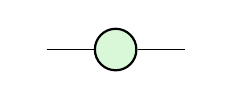
\begin{tikzpicture}
    \node (0) at (0,0) {};
    \node [style=gn] (1) at (1,0) {};
    \node (2) at (2,0) {};
    \draw (0) to (1);
    \draw (1) to (2);
  \end{tikzpicture}\\
  Očitno ne predstavljajo več unitarnih preslikav
\end{frame}
\begin{frame}
  \frametitle{Hadamardova vrata}
  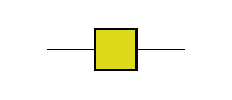
\begin{tikzpicture}
    \node (0) at (0,0) {};
    \node [style=had] (1) at (1,0) {};
    \node (2) at (2,0) {};
    \draw (0) to (1);
    \draw (1) to (2);
  \end{tikzpicture}\\
  Hadamardova vrata spreminjajo bazo. Lahko definiramo kot kompozicijo Z in X pajkov\\
  \vspace{3mm}
  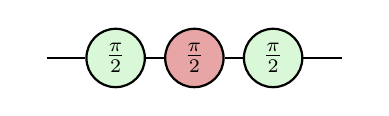
\begin{tikzpicture}
    \node (0) at (0.00, 0.00) {};
    \node [style=gn] (1) at (1, 0) {\(\frac\pi2\)};
    \node [style=rn] (2) at (2, 0) {\(\frac\pi2\)};
    \node [style=gn] (3) at (3, 0) {\(\frac\pi2\)};
    \node (4) at (4.00, 0.00) {};
    \draw (0) to (1);
    \draw (1) to (2);
    \draw (2) to (3);
    \draw (3) to (4);
  \end{tikzpicture}\\\pause{}
  Če imamo\vspace{3mm}\\
  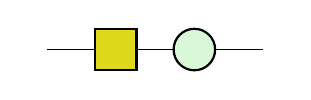
\begin{tikzpicture}
    \node (0) at (0,0) {};
    \node [style=had] (1) at (1,0) {};
    \node [style=gn] (2) at (2,0) {};
    \node (3) at (3,0) {};
    \draw (0) to (1);
    \draw (1) to (2);
    \draw (2) to (3);
  \end{tikzpicture}\\
  Lahko to pretvorimo v\vspace{3mm}\\
  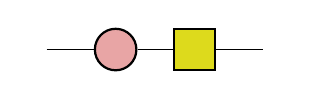
\begin{tikzpicture}
  \node (0) at (0,0) {};
  \node [style=rn] (1) at (1,0) {};
  \node [style=had] (2) at (2,0) {};
  \node (3) at (3,0) {};
  \draw (0) to (1);
  \draw (1) to (2);
  \draw (2) to (3);    
  \end{tikzpicture}
\end{frame}
\begin{frame}
  \frametitle{Povezava s kvantnimi vezji}
  V klasičnih vezjih vrata Z opazujejo spin v Z smeri.\\
  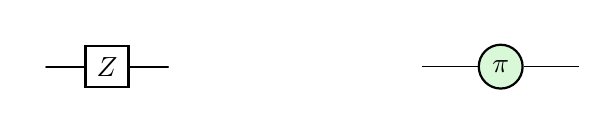
\begin{tikzpicture}
    \node[scale=1.0] (0,0) {
      \begin{quantikz}
        \qw & \gate{Z} & \qw
      \end{quantikz}
    };
    \node [style=gn] (1) at (5,0) {\(\pi\)};
    \draw (4,0) to (1);
    \draw (1) to (6,0);
  \end{tikzpicture}\\
  V ZX-računu to dosežemo s pajkom Z (in \(\alpha=\pi\)). Podobno za X smer.\\
  Vrata C-NOT postanejo\vspace{3mm}\\
  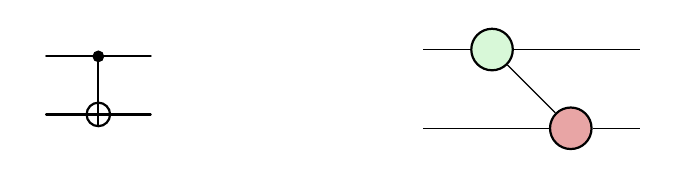
\begin{tikzpicture}
    \node (quantum) at (0,0.5) {
      \begin{quantikz}
        \qw & \ctrl{1} & \qw \\
        \qw & \targ{}  & \qw
      \end{quantikz}
    };
    \node (0) at (4, 0.00) {};
    \node (1) at (4, 1.00) {};
    \node [style=gn] (3) at (5, 1.00) {};
    \node [style=rn] (2) at (6, 0.00) {};
    \node (4) at (7, 0.00) {};
    \node (5) at (7, 1.00) {};
    \draw (0) to (2);
    \draw (1) to (3);
    \draw (2) to (3);
    \draw (2) to (4);
    \draw (3) to (5);
  \end{tikzpicture}\\
  Zgornji kubit pusti nespremenjen, spodnjega negira.
\end{frame}
\begin{frame}
  Klasično kvantno vezje od prej
  \begin{center}
  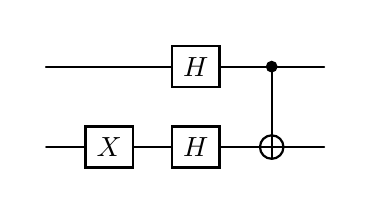
\begin{tikzpicture}
    \node[scale=1.0] {
      \begin{quantikz}
        \qw & \qw       & \gate{H} & \ctrl{1} & \qw \\
        \qw & \gate{X}  & \gate{H} & \targ{}  & \qw
      \end{quantikz}
    };
  \end{tikzpicture}
\end{center}
lahko pretvorimo v
\begin{center}
  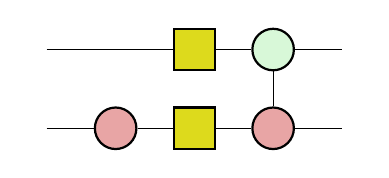
\begin{tikzpicture}
    \node (1) at (0,1) {};
    \node (0) at (0,0) {};
    \node [style=rn] (x) at (1,0) {};
    \node [style=had] (up) at (2,1) {};
    \node [style=had] (down) at (2,0) {};
    \node [style=rn] (cnotr) at (3,0) {};
    \node [style=gn] (cnotg) at (3,1) {};
    \node (11) at (4,1) {};
    \node (10) at (4,0) {};
    \draw (1) to (up);
    \draw (0) to (x);
    \draw (x) to (down);
    \draw (down) to (cnotr);
    \draw (up) to (cnotg);
    \draw (cnotg) to (cnotr);
    \draw (cnotr) to (10);
    \draw (cnotg) to (11);
  \end{tikzpicture}
\end{center}
\end{frame}
\begin{frame}
  \frametitle{Pravila}
  Postavimo si nekaj aksiomov, s katerimi grafično poenostavljamo vezja.

  Izbira ni unikatna! Z izbiro aksiomov izberemo delec ZX-računa. S tem izberemo kakšne kvantne sisteme simulira.

  Namesto, da izhajamo iz negativnih trditev (kvantna teorija mere izhaja iz \emph{ne}aditivnosti meritev, kvantna logika iz \emph{ne}distributivnosti\dots), izhajamo iz pozitivnih (kaj velja).
\end{frame}
\begin{frame}
  \frametitle{Uvod v aksiome}
  Vsako pravilo velja če zamenjamo vse barve.

  Graf lahko topološko preuredimo in še vedno predstavlja isti sistem (fiksiramo le globalne vhode in izhode)
\end{frame}
\begin{frame}
  \frametitle{Aksiom: Pajki}
  Povezane pajke iste barve lahko združimo in seštejemo fazo.\\
  \begin{center}
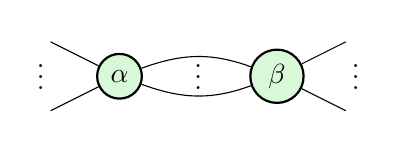
\begin{tikzpicture}
    \node (00) at (0,0) {};
    \node (dots1) at (0, 0.6) {\vdots};
    \node (01) at (0,1) {};
    \node [style=gn] (first) at (1,0.5) {\(\alpha\)};
    \node [style=gn] (second) at (3,0.5) {\(\beta\)};
    \node (dots3) at (2,0.6) {\vdots};
    \node (10) at (4,0) {};
    \node (dots2) at (4,0.6) {\vdots};
    \node (11) at (4,1) {};
    \draw (00) to (first);
    \draw (01) to (first);
    \draw (first) to [in=160, out=20] (second);
    \draw (first) to [in=200, out=340] (second);
    \draw (second) to (10);
    \draw (second) to (11);
  \end{tikzpicture}
\end{center}
  Je ekvivalenten
  \begin{center}
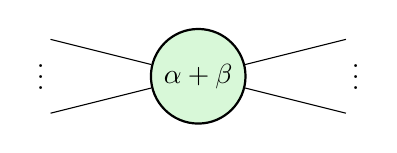
\begin{tikzpicture}
    \node (00) at (-1,0) {};
    \node (dots1) at (-1, 0.6) {\vdots};
    \node (01) at (-1,1) {};
    \node [style=gn] (first) at (1,0.5) {\(\alpha+\beta\)};
    \node (10) at (3,0) {};
    \node (dots2) at (3,0.6) {\vdots};
    \node (11) at (3,1) {};
    \draw (00) to (first);
    \draw (01) to (first);
    \draw (first) to (10);
    \draw (first) to (11);
  \end{tikzpicture}
\end{center}
\end{frame}
\begin{frame}
  \frametitle{Aksiom: Identiteta}
  \begin{center}
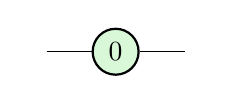
\begin{tikzpicture}
    \node (0) at (0,0) {};
    \node [style=gn] (g) at (1,0) {\(0\)};
    \node (1) at (2,0) {};
    \draw (0) to (g);
    \draw (g) to (1);
  \end{tikzpicture}
\end{center}
  Je ekvivalenten
  \begin{center}
\begin{tikzpicture}
    \node (0) at (0,0) {};
    \node (1) at (2,0) {};
    \draw (0) to (1);
  \end{tikzpicture}
\end{center}
\end{frame}
\begin{frame}
  \frametitle{Primer: inverzi}
  Inverzne faze: \(-\alpha\) je inverzna faza od \(\alpha\)
  \begin{center}
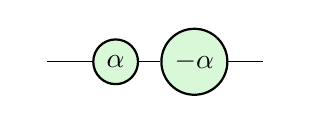
\begin{tikzpicture}
    \node (0) at (0,0) {};
    \node [style=gn] (1) at (1,0) {\(\alpha\)};
    \node [style=gn] (2) at (2,0) {\(-\alpha\)};
    \node (3) at (3,0) {};
    \draw (0) to (1);
    \draw (1) to (2);
    \draw (2) to (3);
  \end{tikzpicture}
\end{center}
\end{frame}
\begin{frame}
  \frametitle{Primer: inverzi}
  Inverzne faze: \(-\alpha\) je inverzna faza od \(\alpha\)
  \begin{center}
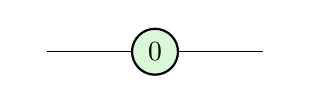
\begin{tikzpicture}
    \node (0) at (0,0) {};
    \node [style=gn] (1) at (1.5,0) {\(0\)};
    \node (3) at (3,0) {};
    \draw (0) to (1);
    \draw (1) to (3);
  \end{tikzpicture}
\end{center}
\end{frame}
\begin{frame}
  \frametitle{Primer: inverzi}
  Inverzne faze: \(-\alpha\) je inverzna faza od \(\alpha\)
  \begin{center}
\begin{tikzpicture}
    \node (0) at (0,0) {};
    \node (3) at (3,0) {};
    \draw (0) to (3);
  \end{tikzpicture}
\end{center}
\end{frame}
\begin{frame}
  \frametitle{Primer: odstranjevanje zank}
  \begin{center}
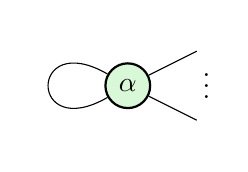
\begin{tikzpicture}
    \node [style=gn](main) at (1,0.5) {\(\alpha\)};
    \node (1) at (2,0) {};
    \node (dots) at (2,0.6) {\vdots};
    \node (2) at (2,1) {};
    \draw (main) to (1);
    \draw (main) to (2);
    \draw (main) to [in=150, out=210, looseness=10] (main);
  \end{tikzpicture}
\end{center}
  Je ekvivalentna
  \begin{center}
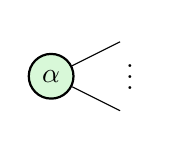
\begin{tikzpicture}
    \node [style=gn](main) at (1,0.5) {\(\alpha\)};
    \node (1) at (2,0) {};
    \node (dots) at (2,0.6) {\vdots};
    \node (2) at (2,1) {};
    \draw (main) to (1);
    \draw (main) to (2);
  \end{tikzpicture}
\end{center}
\end{frame}
\begin{frame}
  \frametitle{Aksiom: Bialgebra}
  \begin{center}
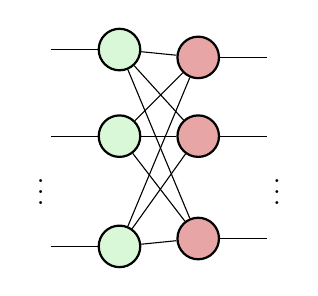
\begin{tikzpicture}
    \node (1s) at (0,0) {};
    \node (dotss) at (0, 0.8) {\vdots};
    \node (2s) at (0,1.4) {};
    \node (3s) at (0,2.5) {};
    \node [style=gn] (1g) at (1,0) {};
    \node [style=gn] (2g) at (1,1.4) {};
    \node [style=gn] (3g) at (1,2.5) {};
    \node [style=rn] (1r) at (2,0.1) {};
    \node [style=rn] (2r) at (2,1.4) {};
    \node [style=rn] (3r) at (2,2.4) {};
    \node (1e) at (3,0.1) {};
    \node (2e) at (3,1.4) {};
    \node (dotse) at (3, 0.8) {\vdots};
    \node (3e) at (3,2.4) {};
    \draw (1s) to (1g);
    \draw (2s) to (2g);
    \draw (3s) to (3g);
    \draw (1g) to (1r);
    \draw (1g) to (2r);
    \draw (1g) to (3r);
    \draw (2g) to (1r);
    \draw (2g) to (2r);
    \draw (2g) to (3r);
    \draw (3g) to (1r);
    \draw (3g) to (2r);
    \draw (3g) to (3r);
    \draw (1r) to (1e);
    \draw (2r) to (2e);
    \draw (3r) to (3e);
  \end{tikzpicture}
\end{center}
  Je ekvivalenten
  \begin{center}
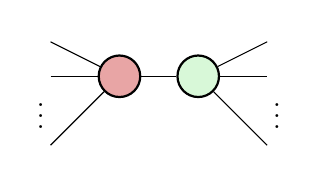
\begin{tikzpicture}
    \node (1s) at (0,0) {};
    \node (dotss) at (0, 0.6) {\vdots};
    \node (2s) at (0,1) {};
    \node (3s) at (0,1.5) {};
    \node [style=rn] (g) at (1, 1) {};
    \node [style=gn] (r) at (2, 1) {};
    \node (1e) at (3,0) {};
    \node (2e) at (3,1) {};
    \node (dotse) at (3, 0.6) {\vdots};
    \node (3e) at (3,1.5) {};
    \draw (1s) to (g);
    \draw (2s) to (g);
    \draw (3s) to (g);
    \draw (g) to (r);
    \draw (r) to (1e);
    \draw (r) to (2e);
    \draw (r) to (3e);
  \end{tikzpicture}
\end{center}
\end{frame}
\begin{frame}
  \frametitle{Primer: Kopiranje}
  Kopiranje (posebni primer bialgebre, ko ima pajek 0 povezav)
  \begin{center}
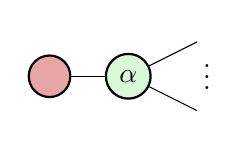
\begin{tikzpicture}
    \node [style=rn] (origin) at (0,0.5) {};
    \node [style=gn] (mid) at (1,0.5) {\(\alpha\)};
    \node (end) at (2,0) {};
    \node (dots) at (2,0.6) {\vdots};
    \node (end2) at (2,1) {};
    \draw (origin) to (mid);
    \draw (mid) to (end);
    \draw (mid) to (end2);
  \end{tikzpicture}
\end{center}
  postane
  \begin{center}
    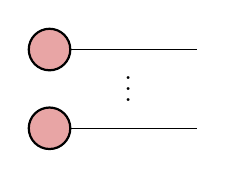
\begin{tikzpicture}
      \node [style=rn] (1) at (0,0) {};
      \node (1e) at (2,0) {};
      \node (dots) at (1,0.6) {\vdots};
      \node [style=rn] (2) at (0,1) {};
      \node (2e) at (2,1) {};
      \draw (1) to (1e);
      \draw (2) to (2e);
    \end{tikzpicture}
  \end{center}
  To pravilo predstavlja nekvantne podatke.
\end{frame}
\begin{frame}
  \frametitle{Primer: Komplementarnost}
  Želimo poenostaviti
  \begin{center}
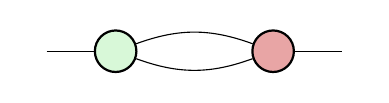
\begin{tikzpicture}
    \node (00) at (0,0.5) {};
    \node [style=gn] (first) at (1,0.5) {};
    \node [style=rn] (second) at (3,0.5) {};
    \node (10) at (4,0.5) {};
    \draw (00) to (first);
    \draw (first) to [in=160, out=20] (second);
    \draw (first) to [in=200, out=340] (second);
    \draw (second) to (10);
  \end{tikzpicture}
\end{center}
\end{frame}
\begin{frame}
  \frametitle{Primer: Komplementarnost}
  Samotni pajek je identiteta
  \begin{center}
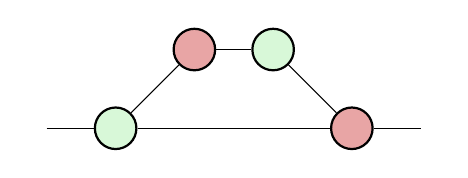
\begin{tikzpicture}
    \node (00) at (0,0) {};
    \node [style=rn] (imd) at (2,1) {};
    \node [style=gn] (imd2) at (3,1) {};
    \node [style=gn] (first) at (1,0) {};
    \node [style=rn] (second) at (4,0) {};
    \node (10) at (5,0) {};
    \draw (00) to (first);
    \draw (first) to (second);
    \draw (second) to (10);
    \draw (first) to (imd);
    \draw (imd) to (imd2);
    \draw (imd2) to (second);
  \end{tikzpicture}
\end{center}
\end{frame}
\begin{frame}
  \frametitle{Primer: Komplementarnost}
  Topološko ekvivalentno vezje je ekvivalentno
  \begin{center}
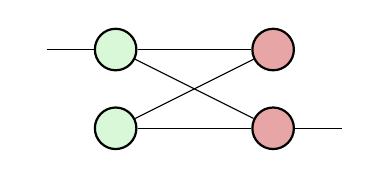
\begin{tikzpicture}
    \node (00) at (0,1) {};
    \node [style=rn] (imd) at (3,1) {};
    \node [style=gn] (imd2) at (1,0) {};
    \node [style=gn] (first) at (1,1) {};
    \node [style=rn] (second) at (3,0) {};
    \node (10) at (4,0) {};
    \draw (00) to (first);
    \draw (first) to (second);
    \draw (second) to (10);
    \draw (first) to (imd);
    \draw (imd) to (imd2);
    \draw (imd2) to (second);
  \end{tikzpicture}
\end{center}
\end{frame}
\begin{frame}
  \frametitle{Primer: Komplementarnost}
  Dodamo nove pajke, ki ne spremenijo vezja
  \begin{center}
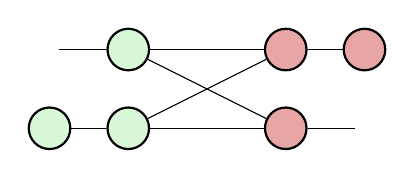
\begin{tikzpicture}
    \node (00) at (0,1) {};
    \node [style=gn] (newg) at (0,0) {};
    \node [style=rn] (newr) at (4,1) {};
    \node [style=rn] (imd) at (3,1) {};
    \node [style=gn] (imd2) at (1,0) {};
    \node [style=gn] (first) at (1,1) {};
    \node [style=rn] (second) at (3,0) {};
    \node (10) at (4,0) {};
    \draw (00) to (first);
    \draw (newr) to (imd);
    \draw (newg) to (imd2);
    \draw (first) to (second);
    \draw (second) to (10);
    \draw (first) to (imd);
    \draw (imd) to (imd2);
    \draw (imd2) to (second);
  \end{tikzpicture}
\end{center}
\end{frame}
\begin{frame}
  \frametitle{Primer: Komplementarnost}
  Uporabimo pravilo bialgebre
  \begin{center}
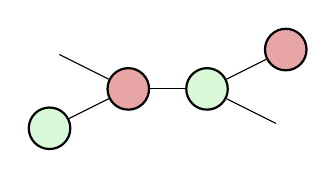
\begin{tikzpicture}
    \node (in) at (0,1) {};
    \node [style=gn] (ing) at (0,0) {};
    \node [style=rn] (mainr) at (1,0.5) {};
    \node [style=gn] (maing) at (2,0.5) {};
    \node (out) at (3,0) {};
    \node [style=rn] (outr) at (3,1) {};
    \draw (in) to (mainr);
    \draw (ing) to (mainr);
    \draw (mainr) to (maing);
    \draw (maing) to (out);
    \draw (maing) to (outr);
  \end{tikzpicture}
\end{center}
\end{frame}
\begin{frame}
  \frametitle{Primer: Komplementarnost}
  Spet topološko preuredimo za boljšo preglednost
  \begin{center}
  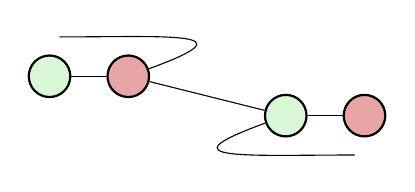
\begin{tikzpicture}
    \node (in) at (0,1.5) {};
    \node (out) at (4,0) {};
    \node [style=gn] (ing) at (0,1) {};
    \node [style=rn] (mainr) at (1,1) {};
    \node [style=gn] (maing) at (3,0.5) {};
    \node [style=rn] (outr) at (4,0.5) {};
    \draw (ing) to (mainr);
    \draw (mainr) to (maing);
    \draw (maing) to (outr);
    \draw (in) to [in=20, out=0, looseness=3] (mainr); %\draw (main) to [in=150, out=210, looseness=10] (main);
    \draw (maing) to [in=180, out=200, looseness=3] (out);
  \end{tikzpicture}
\end{center}
\end{frame}
\begin{frame}
  \frametitle{Primer: Komplementarnost}
  Uporabimo izrek za kloniranje na obeh straneh
  \begin{center}
    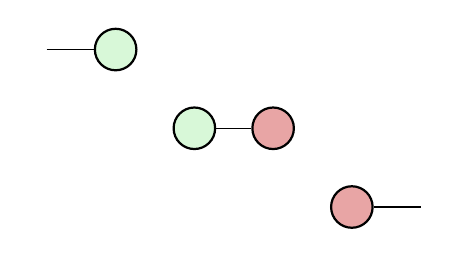
\begin{tikzpicture}
    \node (in) at (0,1) {};
    \node [style=gn] (ing) at (1,1) {};
    \node [style=gn] (middleg) at (2,0) {};
    \node [style=rn] (middler) at (3,0) {};
    \node [style=rn] (outr) at (4,-1) {};
    \node (out) at (5,-1) {};
    \draw (in) to (ing);
    \draw (middleg) to (middler);
    \draw (outr) to (out);
  \end{tikzpicture}
\end{center}
\end{frame}
\begin{frame}
  \frametitle{Primer: Komplementarnost}
  Odstranimo nepovezan del in dobimo, da se
  \begin{center}
    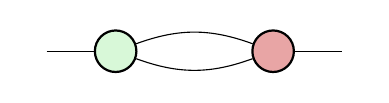
\begin{tikzpicture}
    \node (00) at (0,0.5) {};
    \node [style=gn] (first) at (1,0.5) {};
    \node [style=rn] (second) at (3,0.5) {};
    \node (10) at (4,0.5) {};
    \draw (00) to (first);
    \draw (first) to [in=160, out=20] (second);
    \draw (first) to [in=200, out=340] (second);
    \draw (second) to (10);
  \end{tikzpicture}
\end{center}
  poenostavi v
  \begin{center}
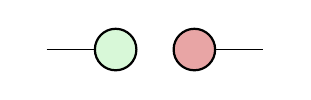
\begin{tikzpicture}
    \node (0) at (0,0) {};
    \node [style=gn] (gn) at (1,0) {};
    \node [style=rn] (rn) at (2,0) {};
    \node (1) at (3,0) {};
    \draw (0) to (gn);
    \draw (rn) to (1);
  \end{tikzpicture}
\end{center}
\end{frame}
\begin{frame}
  \frametitle{Aksiom: Zamenjava barve}
  \begin{center}
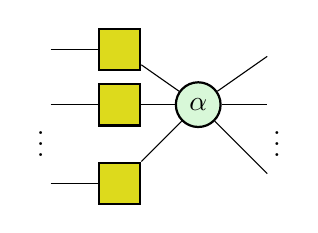
\begin{tikzpicture}
    \node (1s) at (0,0) {};
    \node (dotss) at (0, 0.6) {\vdots};
    \node (2s) at (0,1) {};
    \node (3s) at (0,1.7) {};
    \node [style=had] (1h) at (1,0) {};
    \node [style=had] (2h) at (1,1) {};
    \node [style=had] (3h) at (1,1.7) {};
    \node [style=gn] (main) at (2,1) {\(\alpha\)};
    \node (1e) at (3,0) {};
    \node (2e) at (3,1) {};
    \node (dotse) at (3, 0.6) {\vdots};
    \node (3e) at (3,1.7) {};
    \draw (1s) to (1h);
    \draw (2s) to (2h);
    \draw (3s) to (3h);
    \draw (1h) to (main);
    \draw (2h) to (main);
    \draw (3h) to (main);
    \draw (main) to (1e);
    \draw (main) to (2e);
    \draw (main) to (3e);
  \end{tikzpicture}
\end{center}
  Je ekvivalentno
  \begin{center}
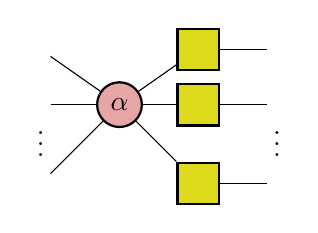
\begin{tikzpicture}
    \node (1s) at (0,0) {};
    \node (dotss) at (0, 0.6) {\vdots};
    \node (2s) at (0,1) {};
    \node (3s) at (0,1.7) {};
    \node [style=had] (1h) at (2,0) {};
    \node [style=had] (2h) at (2,1) {};
    \node [style=had] (3h) at (2,1.7) {};
    \node [style=rn] (main) at (1,1) {\(\alpha\)};
    \node (1e) at (3,0) {};
    \node (2e) at (3,1) {};
    \node (dotse) at (3, 0.6) {\vdots};
    \node (3e) at (3,1.7) {};
    \draw (1s) to (main);
    \draw (2s) to (main);
    \draw (3s) to (main);
    \draw (1h) to (main);
    \draw (2h) to (main);
    \draw (3h) to (main);
    \draw (1h) to (1e);
    \draw (2h) to (2e);
    \draw (3h) to (3e);
  \end{tikzpicture}
\end{center}
\end{frame}
\begin{frame}
  \frametitle{Kvantni orakelj}
  Skoraj vsak zanimiv problem v računalništvu lahko prevedemo v SAT problem.

  Iščemo vrednost \(x\) funkcijske preslikave
  \begin{align*}
    f:\{0,1\}^n\to \{0,1\}
  \end{align*}
  za katero
  \begin{align*}
    f(x) = 1
  \end{align*}
\end{frame}
\begin{frame}
  \frametitle{Kvantni orakelj}
  Predstavili jo bomo z trapezom (da ločimo vhode in izhode)
  \begin{center}
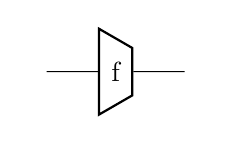
\begin{tikzpicture}
    \node (in) at (0,0) {};
    \node [style=func] (f) at (1,0) {f};
    \node (out) at (2,0) {};
    \draw (in) to (f);
    \draw (f) to (out);
  \end{tikzpicture}
\end{center}
  V splošnem ta funkcija ni unitarna (kar potrebujemo, da predstavlja kvantno vezje)!
\end{frame}
\begin{frame}
  \frametitle{Pogoj homomorfizma}
  Za funkcijske preslikave zahtevamo, da je
  \begin{center}
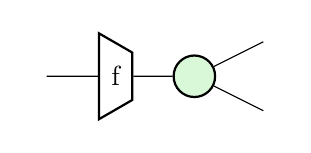
\begin{tikzpicture}
    \node (in) at (0,0) {};
    \node [style=func] (f) at (1,0) {f};
    \node [style=gn] (out) at (2,0) {};
    \node (up) at (3,0.5) {};
    \node (down) at (3,-0.5) {};
    \draw (in) to (f);
    \draw (f) to (out);
    \draw (out) to (up);
    \draw (out) to (down);
  \end{tikzpicture}
\end{center}
  enak
  \begin{center}
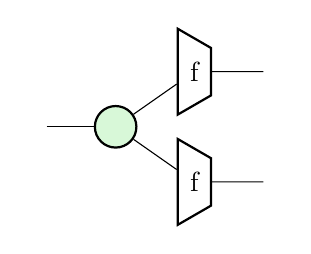
\begin{tikzpicture}
    \node (in) at (0,0) {};
    \node [style=func] (fu) at (2,0.7) {f};
    \node [style=func] (fd) at (2,-0.7) {f};
    \node [style=gn] (out) at (1,0) {};
    \node (up) at (3,0.7) {};
    \node (down) at (3,-0.7) {};
    \draw (in) to (out);
    \draw (fu) to (out);
    \draw (fd) to (out);
    \draw (fu) to (up);
    \draw (fd) to (down);
  \end{tikzpicture}
\end{center}
  To vedno lahko dosežemo tako, da jo zapišemo kot linearno preslikavo.
\end{frame}
\begin{frame}
  \frametitle{Unitarni kvantni orakelj}
  Vsako tako funkcijo lahko pretvorimo v unitarno
  
  Definiramo si iteriran pajek
  \begin{center}
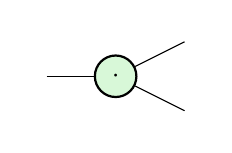
\begin{tikzpicture}
    \node (s) at (0,0) {};
    \node [style=gn] (a) at (1,0) {\(\cdot\)};
    \node (eu) at (2,0.5) {};
    \node (ed) at (2,-0.5) {};
    \draw (s) to (a);
    \draw (a) to (eu);
    \draw (a) to (ed);
  \end{tikzpicture}
\end{center}
  Enak pa naj bo \(n\) kopijam samega sebe brez pike. 
\end{frame}
\begin{frame}
  \frametitle{Unitarni kvantni orakelj}
  Primer za \(n=2\)
  \begin{center}
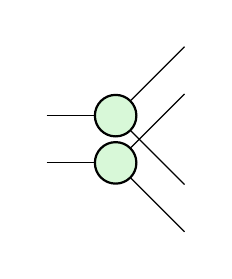
\begin{tikzpicture}
    \node (s) at (0,0) {};
    \node (s2) at (0,0.6) {};
    \node [style=gn] (a) at (1,0) {};
    \node (eu) at (2,1) {};
    \node (ed) at (2,-1) {};
    \node [style=gn] (a2) at (1,0.6) {};
    \node (eu2) at (2,1.6) {};
    \node (ed2) at (2,-0.4) {};
    \draw (s) to (a);
    \draw (a) to (eu);
    \draw (a) to (ed);
    \draw (s2) to (a2);
    \draw (a2) to (eu2);
    \draw (a2) to (ed2);
\end{tikzpicture}
\end{center}
  Vrednost \(n\) je implicitno število vhodov funkcije
\end{frame}
\begin{frame}
  \frametitle{Unitarni kvantni orakelj}
  Preslikava
  \begin{center}
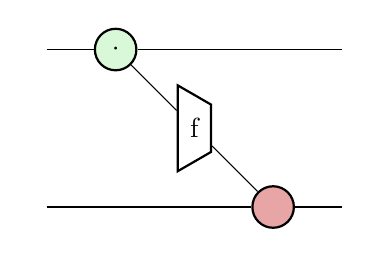
\begin{tikzpicture}
    \node (sr) at (0,0) {};
    \node (sg) at (0,2) {};
    \node [style=gn] (g) at (1,2) {\(\cdot\)};
    \node [style=func] (f) at (2,1) {f};
    \node [style=rn] (r) at (3,0) {};
    \node (eg) at (4,2) {};
    \node (er) at (4,0) {};
    \draw (sg) to (g);
    \draw (g) to (f);
    \draw (f) to (r);
    \draw (g) to (eg);
    \draw (sr) to (r);
    \draw (r) to (er);
\end{tikzpicture}
\end{center}
  je unitarna.
\end{frame}
\begin{frame}
  \frametitle{Unitarni kvantni orakelj}
  Unitarnost lahko potrdimo, da preverimo ali je adjungirana preslikava inverz. V ZX-računu je adjungiran graf kar zrcaljen.
  \begin{center}
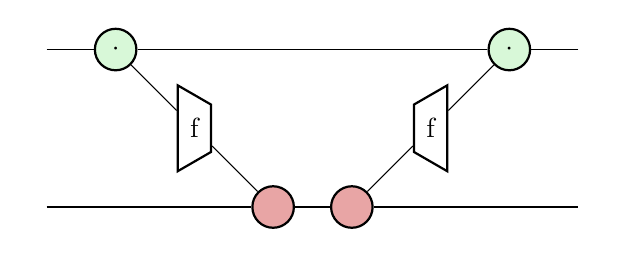
\begin{tikzpicture}
    \node (sr) at (0,0) {};
    \node (sg) at (0,2) {};
    \node [style=gn] (g) at (1,2) {\(\cdot\)};
    \node [style=func] (f) at (2,1) {f};
    \node [style=rn] (r) at (3,0) {};
    \node (sr1) at (7,0) {};
    \node (sg1) at (7,2) {};
    \node [style=gn] (g1) at (6,2) {\(\cdot\)};
    \node [style=func, shape border rotate = 90] (f1) at (5,1) {f};
    \node [style=rn] (r1) at (4,0) {};
    \draw (sg) to (g);
    \draw (g) to (f);
    \draw (f) to (r);
    \draw (g) to (g1);
    \draw (sr) to (r);
    \draw (r) to (r1);
    \draw (sg1) to (g1);
    \draw (g1) to (f1);
    \draw (f1) to (r1);
    \draw (r1) to (sr1);
\end{tikzpicture}
\end{center}
postane 
\begin{center}
  \begin{tikzpicture}
    \node (0) at (0,0) {};
    \node (1) at (0,1) {};
    \node (00) at (7,0) {};
    \node (11) at (7,1) {};
    \draw (0) to (00);
    \draw (1) to (11);
  \end{tikzpicture}
\end{center}
\end{frame}
\begin{frame}
  \frametitle{Kvantni algoritmi}
  Unitarni funkciji določimo vhode in izhode.
  
  Klasični vhod bomo predstavili s trikotnikom
  \begin{center}
    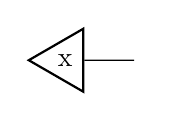
\begin{tikzpicture}
      \node [style=classi] (x) at (0,0) {x};
      \node (o) at (1,0) {};
      \draw (x) to (o);
    \end{tikzpicture}
  \end{center}
\end{frame}
\begin{frame}
  \frametitle{Evalvacija}
  Poglejmo diagram
  \begin{center}
    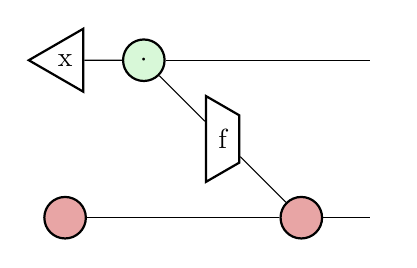
\begin{tikzpicture}
        \node [style=rn] (sr) at (0,0) {};
        \node [style=classi] (sg) at (0,2) {x};
        \node [style=gn] (g) at (1,2) {\(\cdot\)};
        \node [style=func] (f) at (2,1) {f};
        \node [style=rn] (r) at (3,0) {};
        \node (eg) at (4,2) {};
        \node (er) at (4,0) {};
        \draw (sg) to (g);
        \draw (g) to (f);
        \draw (f) to (r);
        \draw (g) to (eg);
        \draw (sr) to (r);
        \draw (r) to (er);
    \end{tikzpicture}
  \end{center}
\end{frame}
\begin{frame}
  \frametitle{Evalvacija}
  Združimo rdeča pajka.
  \begin{center}
    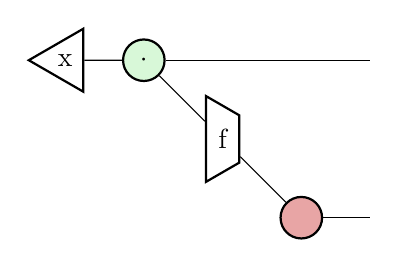
\begin{tikzpicture}
        \node [style=classi] (sg) at (0,2) {x};
        \node [style=gn] (g) at (1,2) {\(\cdot\)};
        \node [style=func] (f) at (2,1) {f};
        \node [style=rn] (r) at (3,0) {};
        \node (eg) at (4,2) {};
        \node (er) at (4,0) {};
        \draw (sg) to (g);
        \draw (g) to (f);
        \draw (f) to (r);
        \draw (g) to (eg);
        \draw (r) to (er);
    \end{tikzpicture}
  \end{center}
\end{frame}
\begin{frame}
  \frametitle{Evalvacija}
  Ker je vhod klasičen se lahko kopira
  \begin{center}
    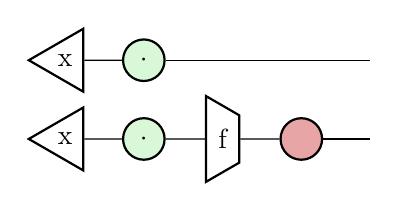
\begin{tikzpicture}
        \node [style=classi] (sg) at (0,2) {x};
        \node [style=classi] (sg2) at (0,1) {x}; 
        \node [style=gn] (g) at (1,2) {\(\cdot\)};
        \node [style=gn] (g2) at (1,1) {\(\cdot\)};
        \node [style=func] (f) at (2,1) {f};
        \node [style=rn] (r) at (3,1) {};
        \node (eg) at (4,2) {};
        \node (er) at (4,1) {};
        \draw (sg) to (g);
        \draw (g2) to (f);
        \draw (f) to (r);
        \draw (g) to (eg);
        \draw (r) to (er);
        \draw (g2) to (sg2);
    \end{tikzpicture}
  \end{center}
\end{frame}
\begin{frame}
  \frametitle{Evalvacija}
  Odstranimo identitete
  \begin{center}
    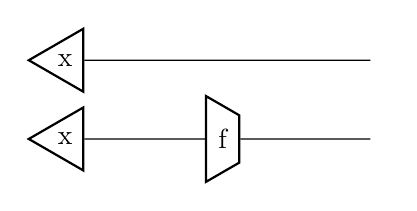
\begin{tikzpicture}
        \node [style=classi] (sg) at (0,2) {x};
        \node [style=classi] (sg2) at (0,1) {x}; 
        \node [style=func] (f) at (2,1) {f};
        \node (eg) at (4,2) {};
        \node (er) at (4,1) {};
        \draw (sg) to (eg);
        \draw (sg2) to (f);
        \draw (f) to (er);
    \end{tikzpicture}
  \end{center}
\end{frame}
\begin{frame}
  \frametitle{Evalvacija}
  Evalviramo funkcijo
  \begin{center}
    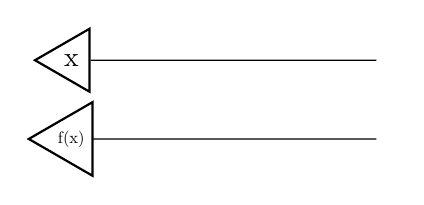
\begin{tikzpicture}
      \node [style=classi] (x) at (0,1) {x};
      \node [style=classi, scale=0.6, inner sep = 1pt] (fx) at (0,0) {f(x)};
      \node (out1) at (4,1) {};
      \node (out2) at (4,0) {};
      \draw (x) to (out1);
      \draw (fx) to (out2);
    \end{tikzpicture}
  \end{center}
  Tako smo pokazali, da je prejšnji diagram dejansko samo evalvacija funkcije!
\end{frame}
\begin{frame}
  \frametitle{Superpozicija vseh vhodov}
  Podobno lahko pokažemo, da je
  \begin{center}
    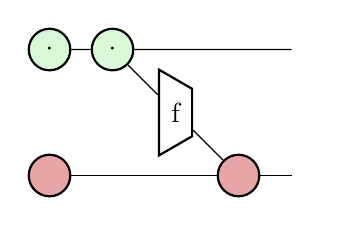
\begin{tikzpicture}[scale=0.8]
        \node [style=rn] (sr) at (0,0) {};
        \node [style=gn] (sg) at (0,2) {\(\cdot\)};
        \node [style=gn] (g) at (1,2) {\(\cdot\)};
        \node [style=func] (f) at (2,1) {f};
        \node [style=rn] (r) at (3,0) {};
        \node (eg) at (4,2) {};
        \node (er) at (4,0) {};
        \draw (sg) to (g);
        \draw (g) to (f);
        \draw (f) to (r);
        \draw (g) to (eg);
        \draw (sr) to (r);
        \draw (r) to (er);
    \end{tikzpicture}
  \end{center}
  enak
  \begin{center}
    \begin{tikzpicture}[scale=0.8]
      \node [style=func] (f) at (1,0) {f};
      \node (1) at (3,1) {};
      \node (11) at (3,0) {};
      \draw (0,0) arc (270:90:0.5);
      \draw (0,0) to (f);
      \draw (f) to (11);
      \draw (0,1) to (1);
    \end{tikzpicture}
  \end{center}
  Kar predstavlja superpozicijo \(f\) na \emph{vseh} vhodih hkrati!
\end{frame}
\begin{frame}
  \frametitle{Problem z vezmi}
  Izkaže se, da splošnega SAT problema ne moremo rešiti (zelo) učinkovito tudi s kvantnimi računalniki.

  Če izmerimo stanje prejšnega vezja, dobimo le vrednost nekega naključnega izhoda.

  Če pa imamo dano kakšno omejitev na funkcijo \(f\), lahko problem rešimo zelo hitro!
\end{frame}
\begin{frame}
  \frametitle{Deutsch-Jozsa algoritem}
  Dano imamo funkcijo
  \begin{align*}
    f: \{0,1\}^n\to \{0,1\},
  \end{align*}
  ki je ali konstantna ali pa uravnotežena, tj. ima točno polovico vhodov \(1\):
  \begin{align*}
    \sum_x f(x) = 2^{n-1}
  \end{align*}
  Ugotoviti želimo ali je konstantna.
\end{frame}
\begin{frame}
  \frametitle{Deutsch-Jozsa algoritem}
  S klasičnimi računalniki moramo funkcijo evalvirati kar \(2^{n-1}+1\) krat! Preverimo več kot polovico vhodov!

  S kvantnim vezjem ugotovimo odgovor v eni sami evalvaciji funkcije.
  \begin{center}
    \begin{tikzpicture}
      \node [style=gn] (sr) at (0,0) {\(\pi\)};
      \node [style=gn] (sg) at (0,2) {\(\cdot\)};
      \node [style=gn] (g) at (1,2) {\(\cdot\)};
      \node [style=func] (f) at (2,1) {f};
      \node [style=rn] (r) at (3,0) {};
      \node [style=gn] (eg) at (4,2) {\(\cdot\)};
      \node [ground, rotate=90] (er) at (4,0) {};
      \draw (sg) to (g);
      \draw (g) to (f);
      \draw (f) to (r);
      \draw (g) to (eg);
      \draw (sr) to (r);
      \draw (r) to (er);
      \draw (eg) to (4.5, 2);
    \end{tikzpicture}
  \end{center}
\end{frame}
\begin{frame}
  \frametitle{Deutsch-Jozsa algoritem}
  Če se vezje poenostavi v
  \begin{center}
    \begin{tikzpicture}
      \node [style=gn] (1) at (0,0) {\(\cdot\)};
      \draw (1) to (1,0);
    \end{tikzpicture}
  \end{center}
  potem je \(f\) konstantna, sicer je uravnotežena.
\end{frame}
\begin{frame}
  \frametitle{Skica dokaza Deutsch-Jozsa}
  Če je funkcija konstantna, izbriše vhod in vnese svojega, torej jo lahko zamenjamo z
  \begin{center}
    \begin{tikzpicture}
      \node (s) at (0,0) {};
      \node [style=gn] (g) at (1,0) {\(\cdot\)};
      \node [style=classi] (x) at (2,0) {x};
      \node (e) at (3,0) {};
      \draw (s) to (g);
      \draw (x) to (e);
    \end{tikzpicture}
  \end{center}
  Dobimo dve ločene komponente. Desno zavržemo, leva se pa poenostavi v željeno meritev
\end{frame}
\begin{frame}
  \frametitle{Skica dokaza Deutsch-Jozsa}
  Če je funkcija ni konstantna, pride v upoštev desna stran. Ko testiramo, če je funkcija konstantna, želimo verjetnost \(0\).
  \begin{center}
    \begin{tikzpicture}
      \node [style=gn] (sr) at (0,0) {\(\pi\)};
      \node [style=gn] (sg) at (0,2) {\(\cdot\)};
      \node [style=gn] (g) at (1,2) {\(\cdot\)};
      \node [style=func] (f) at (2,1) {f};
      \node [style=rn] (r) at (3,0) {};
      \node [style=gn] (eg) at (3.5,2) {\(\cdot\)};
      \node [ground, rotate=90] (er) at (4,0) {};
      \node [style=gn] (const) at (4.5,2) {\(\cdot\)};
      \draw (sg) to (g);
      \draw (g) to (f);
      \draw (f) to (r);
      \draw (g) to (eg);
      \draw (sr) to (r);
      \draw (r) to (er);
      \draw (eg) to (const);
    \end{tikzpicture}
  \end{center}
  Dodamo Z pajek meritve, da preverjamo konstantnost.
\end{frame}
\begin{frame}
  \frametitle{Skica dokaza Deutsch-Jozsa}
  Združimo pajke
  \begin{center}
    \begin{tikzpicture}
      \node [style=gn] (g) at (0,1) {\(\cdot\)};
      \node [style=func] (f) at (2,1) {f};
      \node [style=gn] (sr) at (0,0) {\(\pi\)};
      \node [style=rn] (r) at (3,0) {};
      \node [ground, rotate=90] (er) at (4,0) {};
      \draw (g) to (f);
      \draw (f) to (r);
      \draw (sr) to (r);
      \draw (r) to (er);
    \end{tikzpicture}
  \end{center}
\end{frame}
\begin{frame}
  \frametitle{Skica dokaza Deutsch-Jozsa}
  Pravilo kloniranja
  \begin{center}
    \begin{tikzpicture}
      \node [style=gn] (g) at (0,1) {\(\cdot\)};
      \node [style=func] (f) at (2,1) {f};
      \node [style=gn] (g1) at (3,1) {\(\pi\)};
      \node [style=gn] (g2) at (4,1) {\(\pi\)};
      \node [ground, rotate=90] (er) at (5,1) {};
      \draw (g) to (f);
      \draw (f) to (g1);
      \draw (g2) to (er);
    \end{tikzpicture}
  \end{center}
\end{frame}
\begin{frame}
  \frametitle{Skica dokaza Deutsch-Jozsa}
  Zavržemo del
  \begin{center}
    \begin{tikzpicture}
      \node [style=gn] (g) at (0,1) {\(\cdot\)};
      \node [style=func] (f) at (2,1) {f};
      \node [style=gn] (g1) at (3,1) {\(\pi\)};
      \draw (g) to (f);
      \draw (f) to (g1);
    \end{tikzpicture}
  \end{center}
\end{frame}
\begin{frame}
  \frametitle{Skica dokaza Deutsch-Jozsa}
   Zato na drugem vhodu nastavimo fazo \(\pi\), ker \(e^\pi=-1\). Pajek predstavlja \(\ket0 - \ket 1\)
  \begin{center}
    \begin{tikzpicture}
      \node [classi] (0) at (0,0) {0};
      \node [style=gn] (pi1) at (1,0) {\(\pi\)};
      \node (text) at (2,0) {= 1};
      \node [classi] (1) at (5,0) {1};
      \node [style=gn] (pi2) at (6,0) {\(\pi\)};
      \node (text1) at (7,0) {= -1};
      \draw (0) to (pi1);
      \draw (1) to (pi2);
    \end{tikzpicture}
  \end{center} 
  Če damo funkciji za vhod zelen pajek pa naredi superpozicijo vseh izhodov in jih sešteje. Ker je funkcija uravnotežena, dobimo \(0\).

  Iz tega bi sledilo, da je verjetnost odgovora 0, merili pa smo, če je funkcija konstantna (s predpostavko, da ni).
\end{frame}
\begin{frame}
  \frametitle{Zaključek}
  Za formalen dokaz Deutch-Jozse bi bilo treba definirati podvojena vezja, zavračanje vrednosti in klasične vhode.

  Podoben izgled tudi drugi algoritmi, na primer kvantno iskanje ali iskanje skrite podgrupe.

  Zanimivo področje je tudi računanje preko meritev, še posebej za svetlobna vezja.
\end{frame}
\end{document}